\chapter{Experimental Setting}

The current chapter is divided into two sections. In the first one we will describe the benchmark of the experiment regarding the creation of the RL agent and its results. In the second one we will describe the same experiment applied to humans and its results.

\section{Benchmark}

\paragraph{Test Functions}

As already explained, the experiment described in this work is about maximize black-box functions adopting an RL based approach. The first important choice is about selecting suitable \textit{test functions}. In applied mathematics, test functions, also known as \textit{artificial landscapes}, are useful to evaluate characteristics of optimization algorithms. We have chosen four test functions for this work:

\begin{itemize}
	\item Himmelblau' s Function;
	\item Paraboloid of Revolution;
	\item Beale Function;
	\item Styblinski-Tang' s Revised Function.	
\end{itemize}

\subparagraph{Himmelblau' s Function} In mathematical optimization, Himmelblau' s function is a continuous, bivariate, multi-modal function introduced by David Mautner Himmelblau (1924–2011). The original function is defined by: 

\begin{equation}
	f(x, y) = (x^2 + y -11)^2 + (x + y^2 - 7)^2
\end{equation}

\begin{figure}[h!]
	\centering
	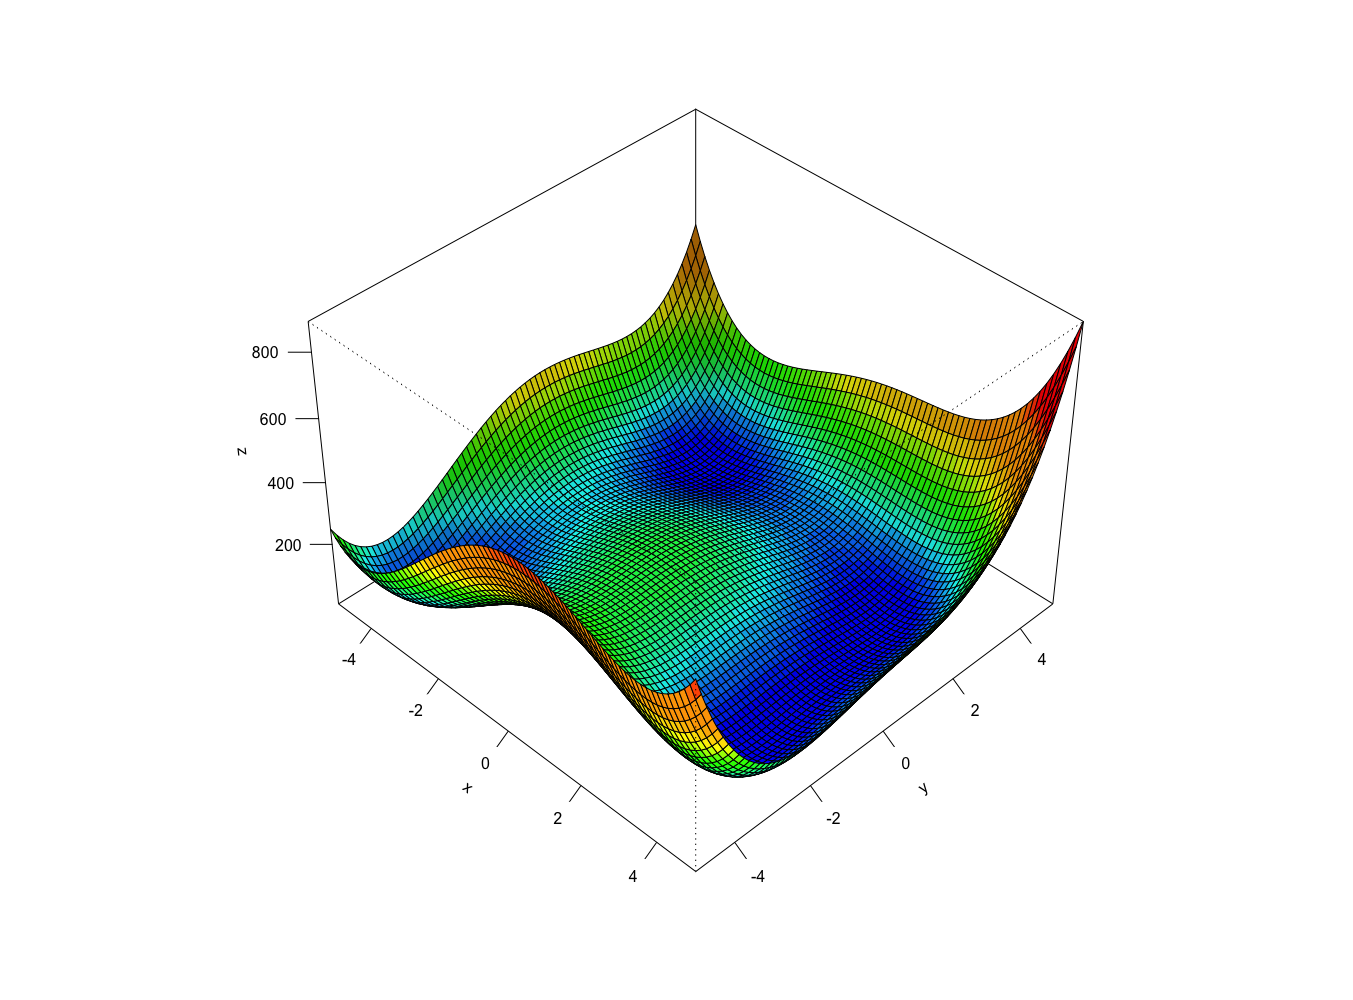
\includegraphics[width= 14cm, height = 14cm]{originalHimmelblau.png}
	\caption{Original Himmelblau' s Function.}
	\label{fig:OriginalHimmelblauFunction}
\end{figure}

It has four local minima :

\begin{itemize}
	\item $f(3.0, 2.0) = 0.0$;
	\item $f(-2.805118, 3.131312) = 0.0$;
	\item $f(-3.779310, -3.283186) = 0.0$;
	\item $f(3.584428, -1848126) = 0.0$.
\end{itemize}
	
The function can be defined on any input domain but it is usually evaluated on $x \in [-5, 5]$ and $y \in [-5, 5]$.

\begin{figure}[h!]
	\centering
	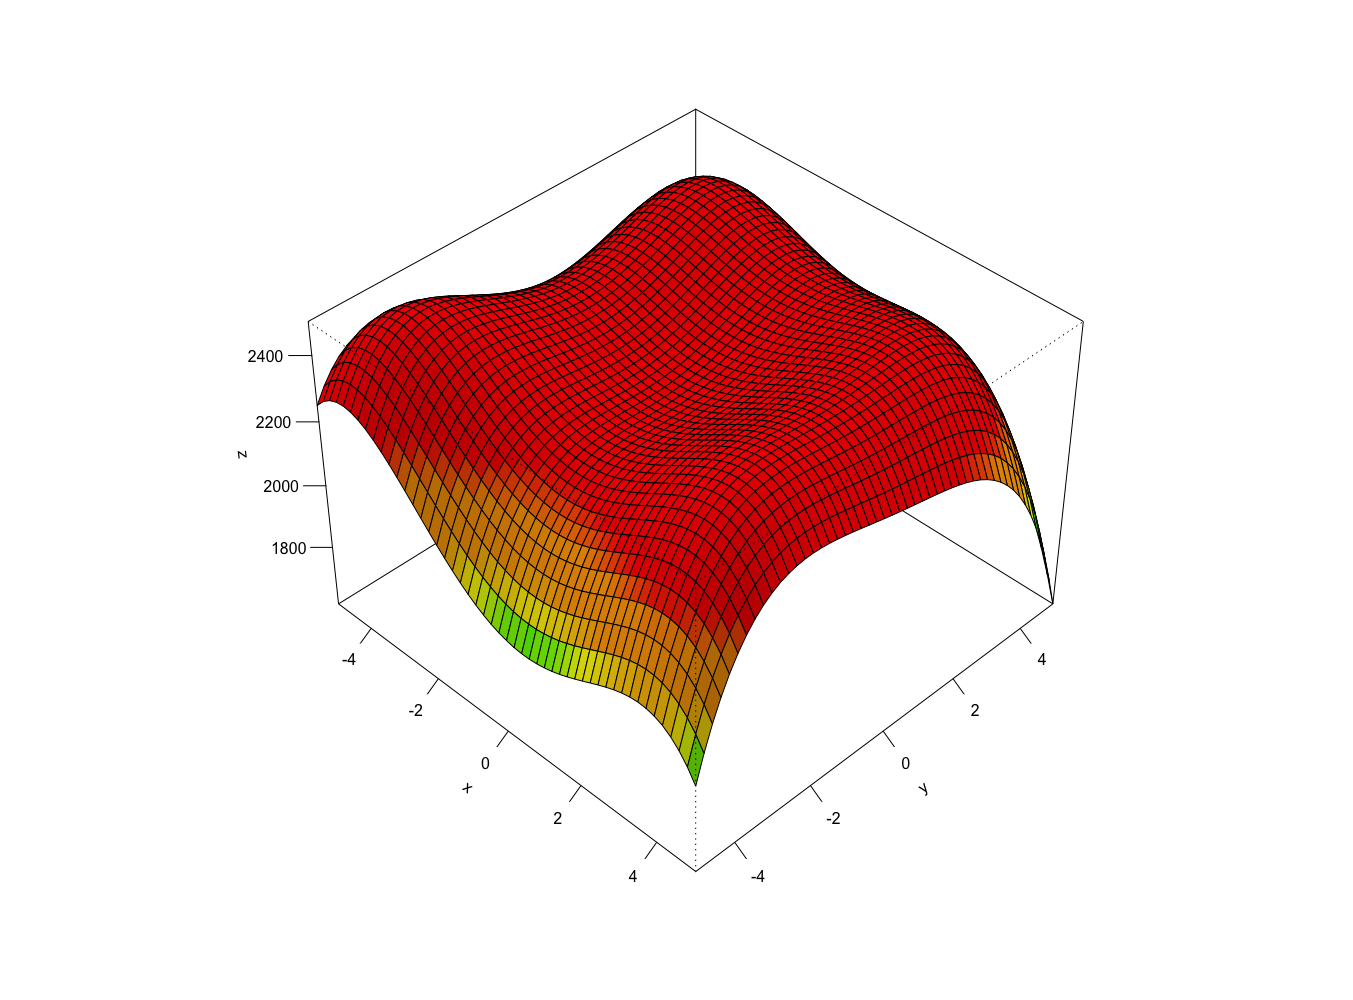
\includegraphics[width= 14cm, height = 14cm]{modifiedHimmelblau.png}
	\caption{Customized Himmelblau' s Function.}
	\label{fig:CustomizedHimmelblauFunction}
\end{figure}

Because of our aim to maximize we inverted the function as follow :

\begin{equation}
f(x, y) = -(x^2 + y -11)^2 + (x + y^2 - 7)^2
\end{equation}

and we picked it up of $2500$ units in order to have as less as possible negative values. So the final adopted function is :
 
\begin{equation}
f(x, y) = -(x^2 + y -11)^2 + (x + y^2 - 7)^2 + 2500
\end{equation}

This function has its global maximum in $f(x, y) = 2500$. \\

In order to represent this customized version of Himmelblau' s Function using Java Graphical Environment, we mapped it in a space of $600 \times 600$ pixels and we properly rotated it. The resulting contour plot is the one represented in figure ~\ref{fig:ContourPlotCustomizedHimmelblauFunction}. \\

\begin{figure}[h!]
	\centering
	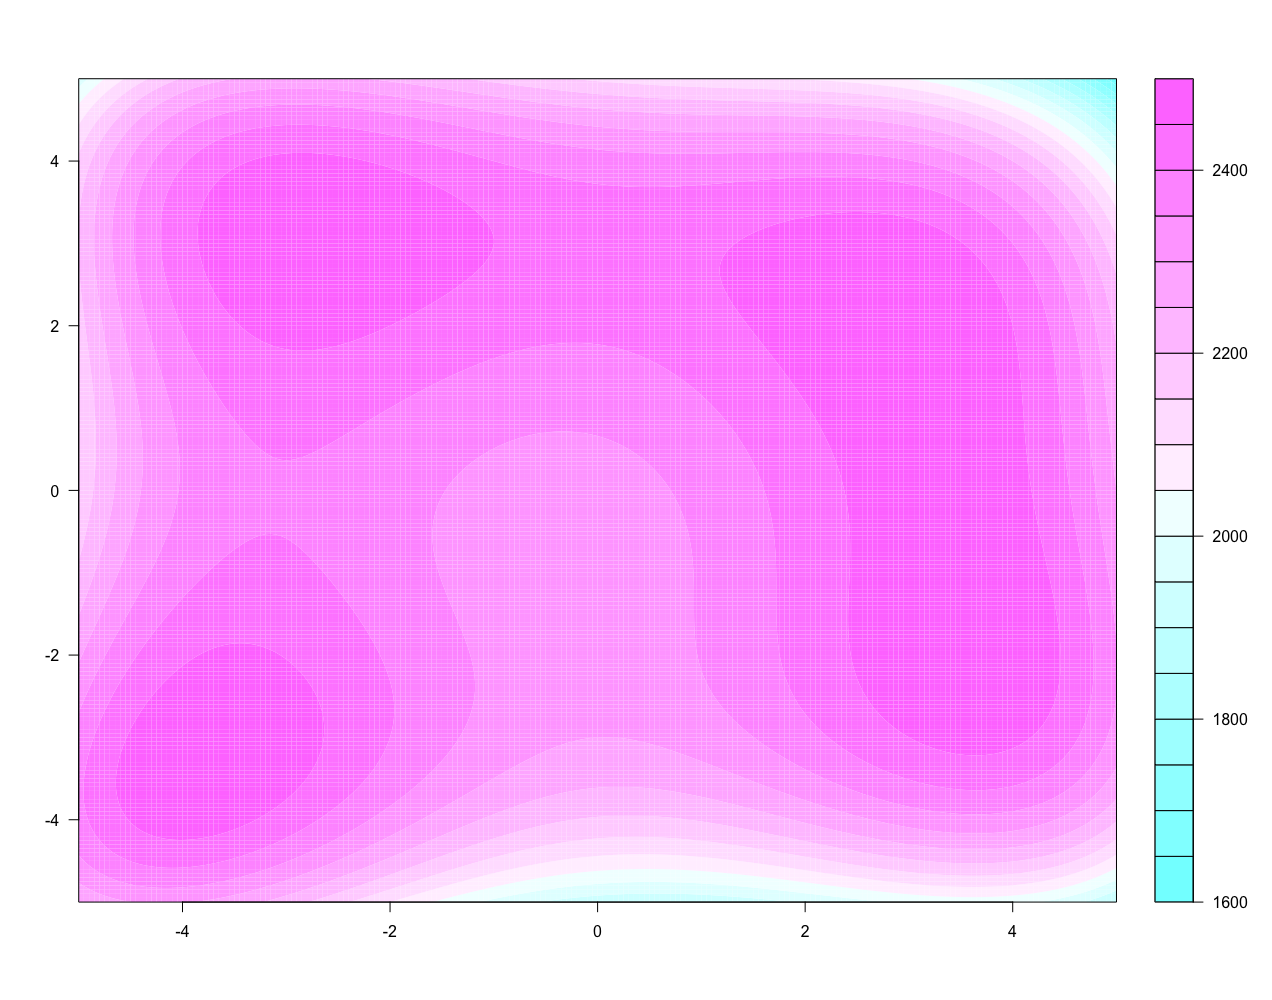
\includegraphics[width= 9cm, height = 9cm]{himmelblau.png}
	\caption{Contour plot of customized version of Himmelblau' s Function.}
	\label{fig:ContourPlotCustomizedHimmelblauFunction}
\end{figure}
 
\subparagraph{Paraboloid of Revolution} In mathematical optimization, Paraboloid of Revolution is a continuous, bivariate, multi-modal function. \\

The original function is defined by: 

\begin{equation}
f(x, y) = (x^2 + y^2) 
\end{equation}

\begin{figure}[h!]
	\centering
	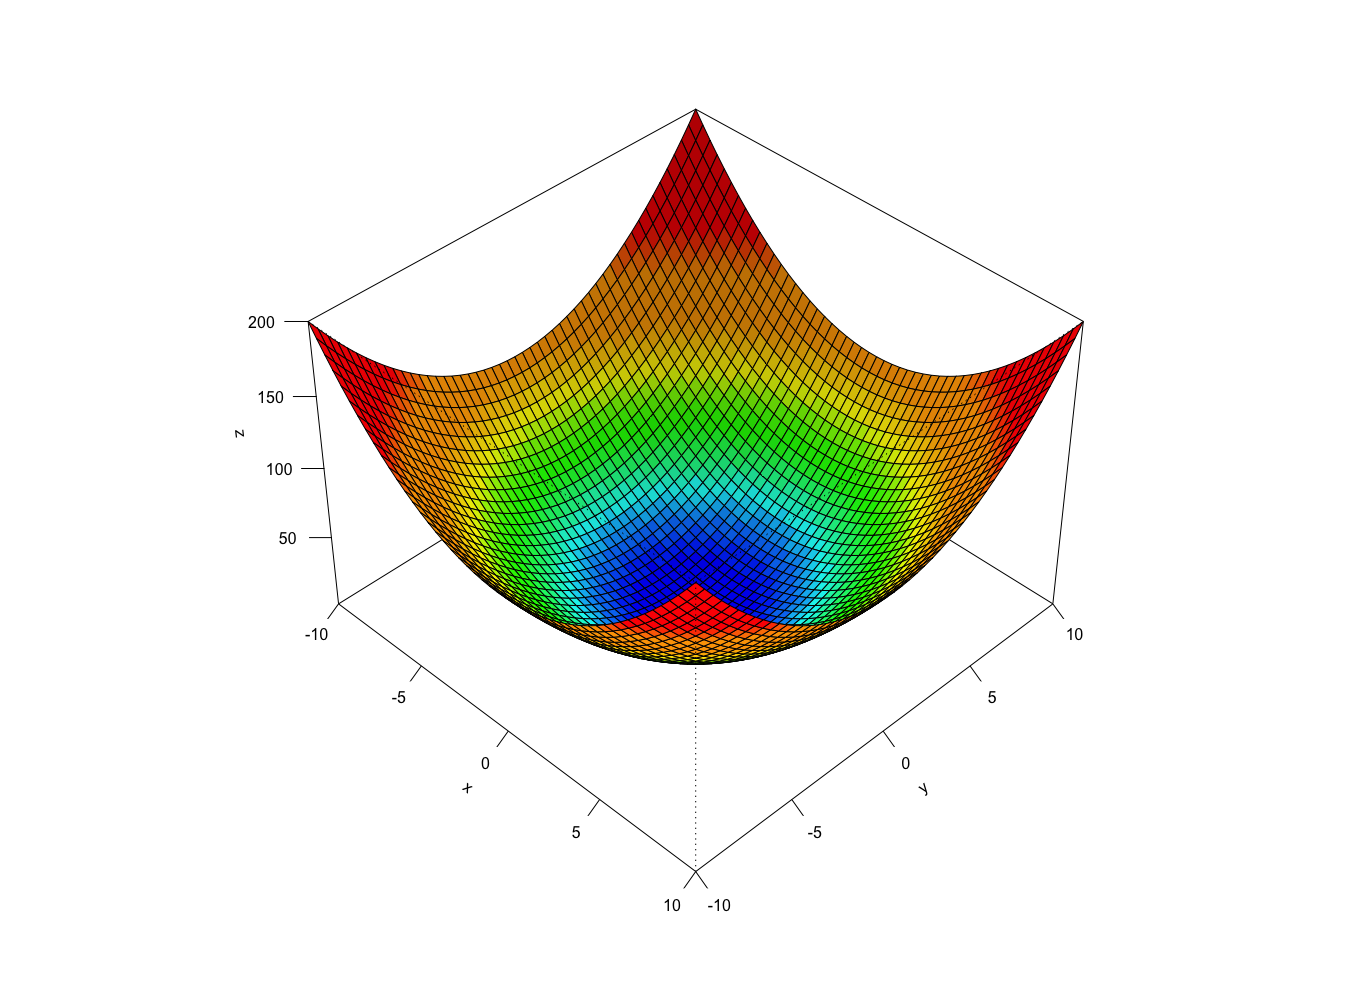
\includegraphics[width= 14cm, height = 14cm]{originalParaboloid.png}
	\caption{Original Paraboloid of Revolution.}
	\label{fig:OriginalParaboloidOfRevolution}
\end{figure}

It has a global minimum in $f(x, y) = 0$. \\

The function can be defined on any input domain but it is usually evaluated on $x \in [-10, 10]$ and $y \in [-10, 10]$. 

\pagebreak

\begin{figure}[h!]
	\centering
	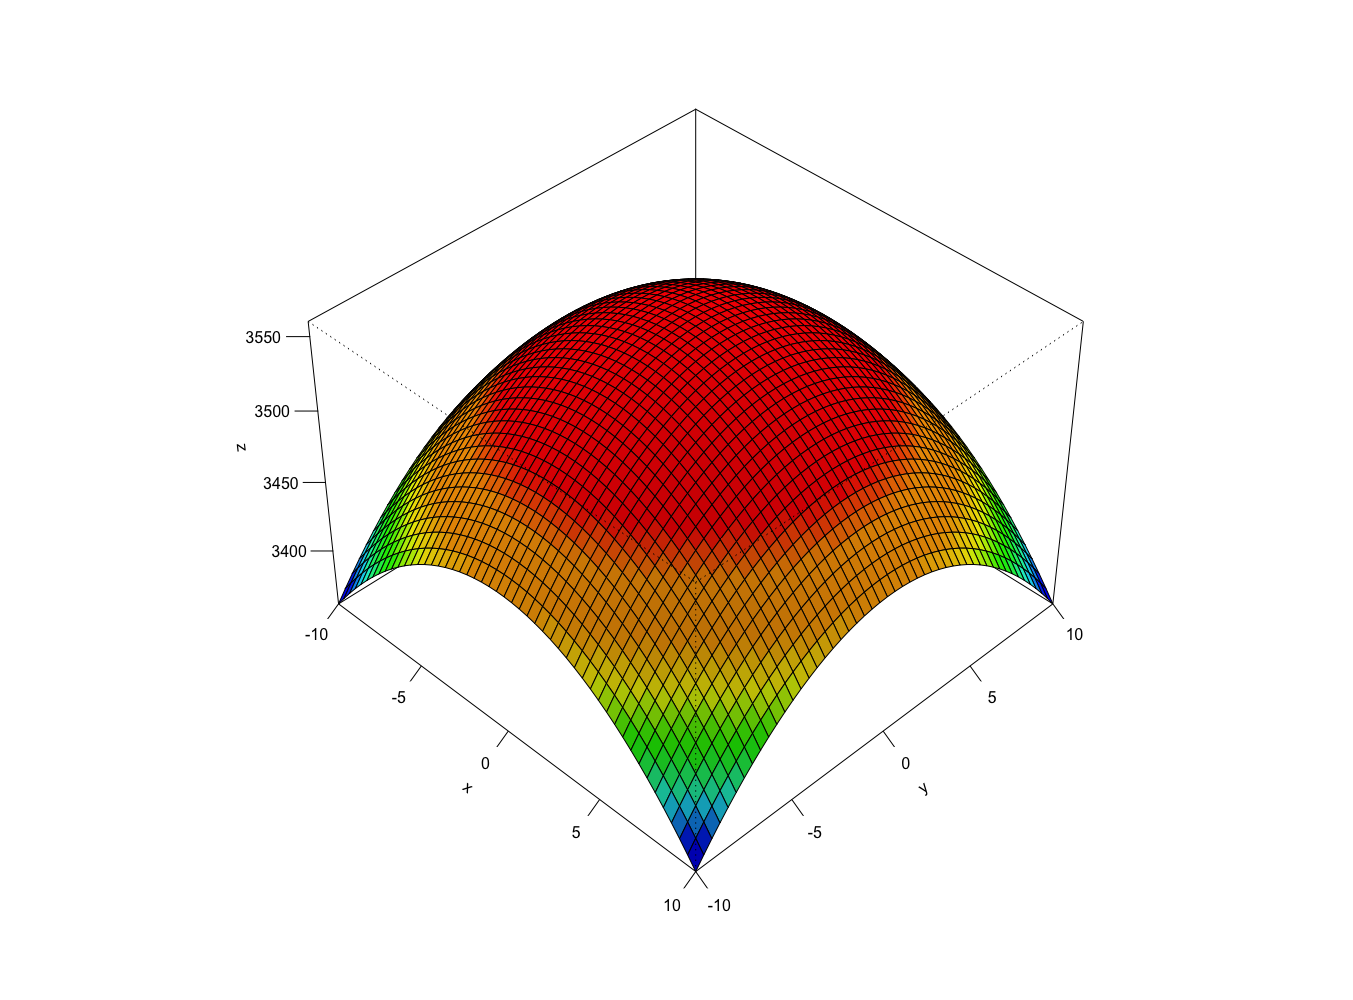
\includegraphics[width= 14cm, height = 14cm]{customizedParaboloid.png}
	\caption{Customized Paraboloid of Revolution.}
	\label{fig:CustomizedParaboloidOfRevolution}
\end{figure}

Because of our aim to maximize, we inverted the function as follow :

\begin{equation}
f(x, y) = -(x^2 + y^2)
\end{equation}

and we picked it up of $3560$ units in order to have as less as possible negative values. So the final adopted function is :

\begin{equation}
f(x, y) = -(x^2 + y^2) + 3560
\end{equation}

This function has its local maximum in $f(x, y) = 3560$.

In order to represent this customized version of Paraboloid of Revolution function using Java Graphical Environment, we mapped it in a space of $600 \times 600$ pixels and we properly rotated it. The resulting contour plot is the one represented in figure ~\ref{fig:ContourPlotCustomizedParabolicFunction} 

\begin{figure}[h!]
	\centering
	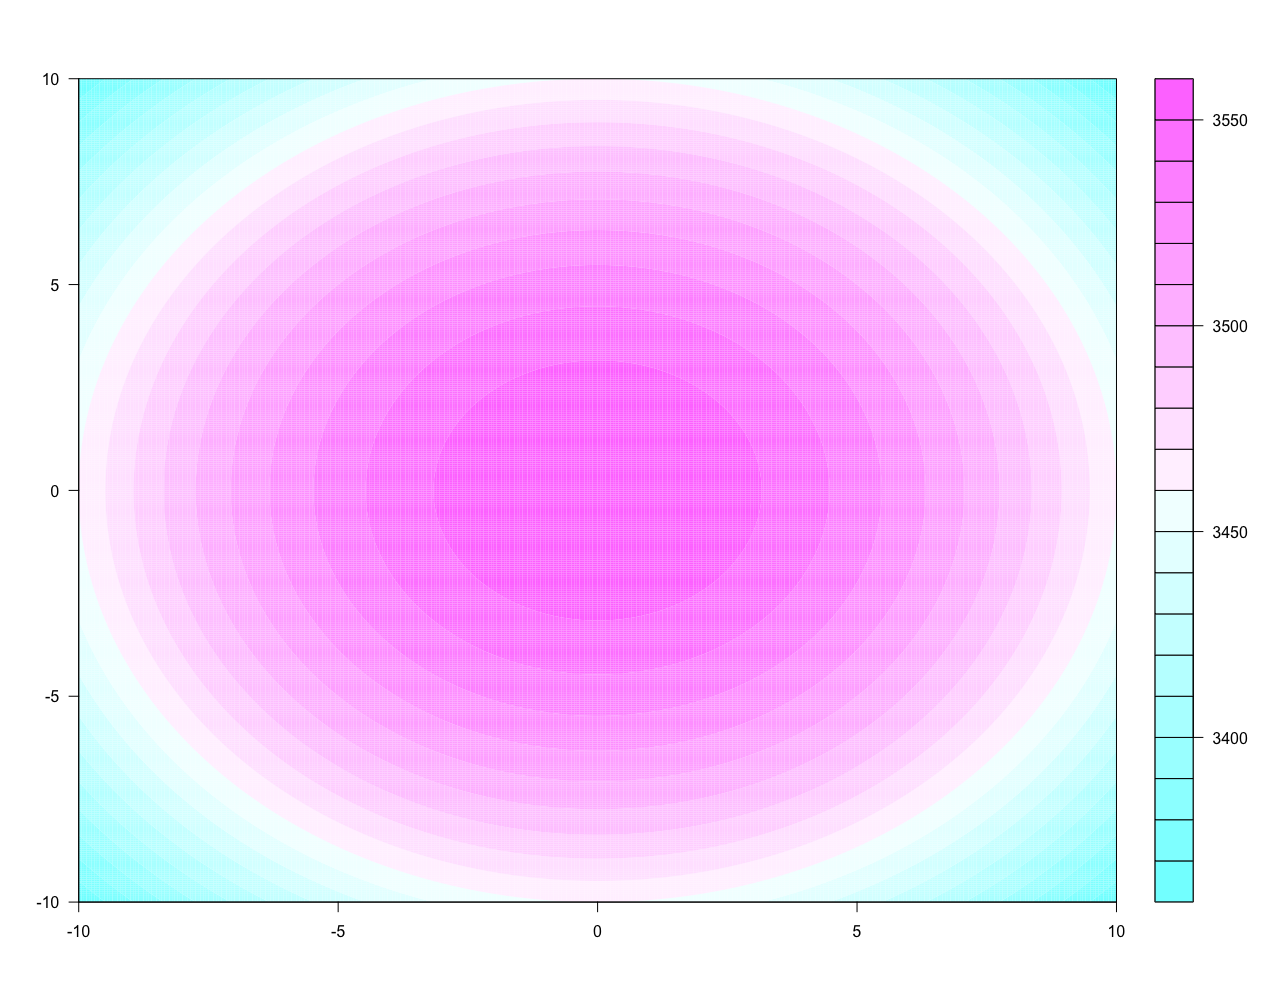
\includegraphics[width= 9cm, height = 9cm]{parabolic.png}
	\caption{Contour plot of customized Parabolic Function.}
	\label{fig:ContourPlotCustomizedParabolicFunction}
\end{figure}

\subparagraph{Beale Function} In mathematical optimization, Beale Function is a continuous, multi-modal function defined on a two-dimensional space. The function is defined by: 

\begin{equation}
f(x, y) = (1.5 - x + xy)^2 + (2.25 - x + xy^2)^2 + (2.625 - x + xy^3)^2
\end{equation}

\break

\begin{figure}[h!]
	\centering
	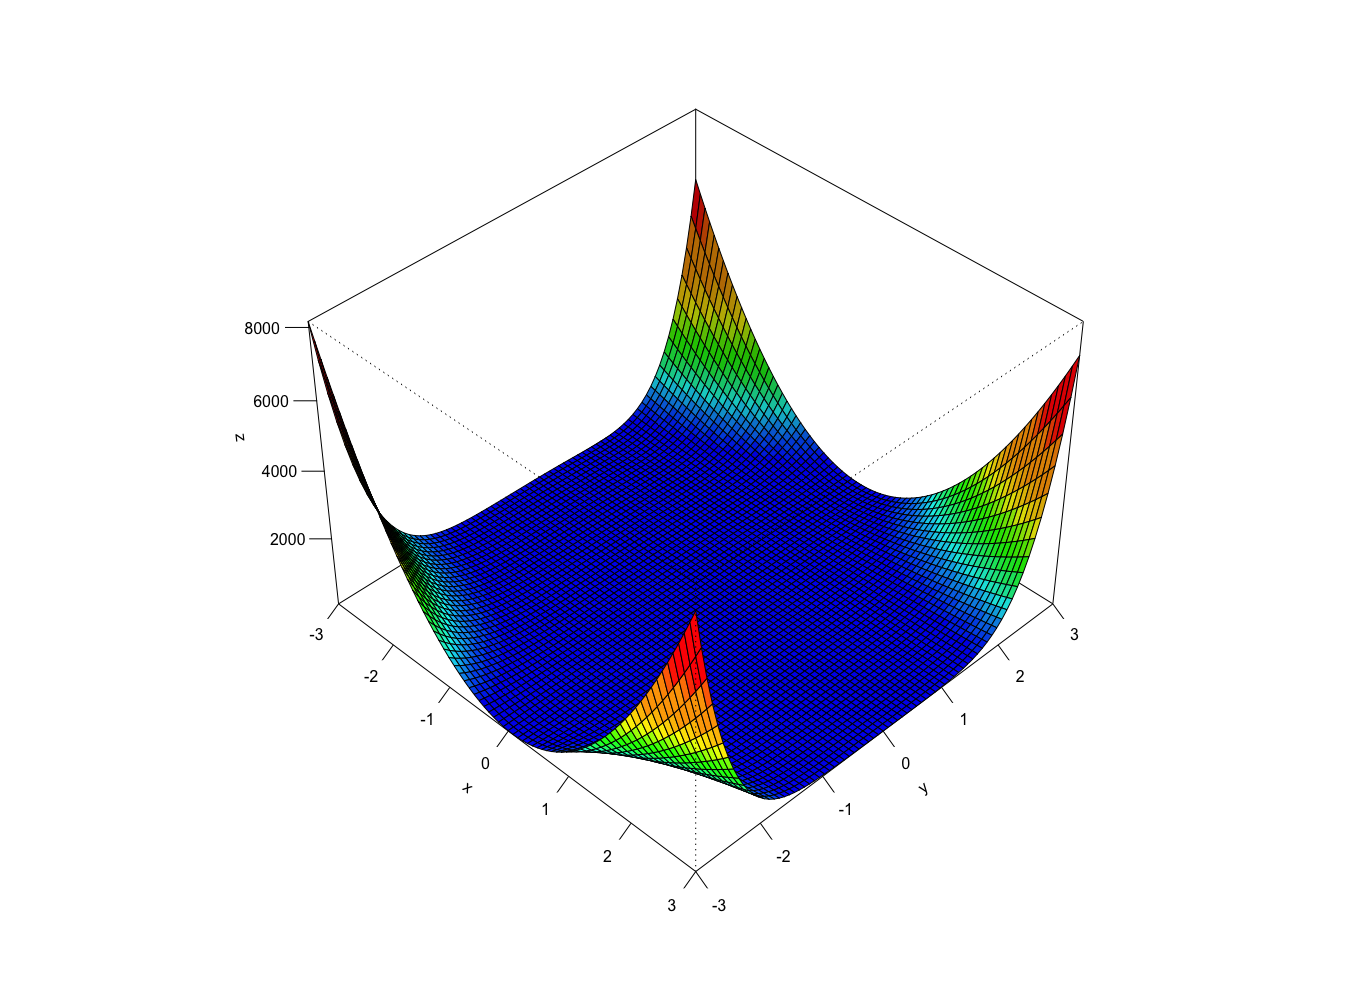
\includegraphics[width= 14cm, height = 14cm]{originalBeale.png}
	\caption{Original Beale Function.}
	\label{fig:OriginalBealeFunction}
\end{figure}

The function can be defined on any input domain but it is usually evaluated on $x \in [-3, 3]$ and $y \in [-3, 3]$. \\

It has one global minimum at: $f(x, y) = 0$. 

In this thesis our aim is to maximize. In order to do this we inverted the function as

\begin{equation}
f(x, y) = -((1.5 - x + xy)^2 + (2.25 - x + xy^2)^2 + (2.625 - x + xy^3)^2)
\end{equation}

\begin{figure}[h!]
	\centering
	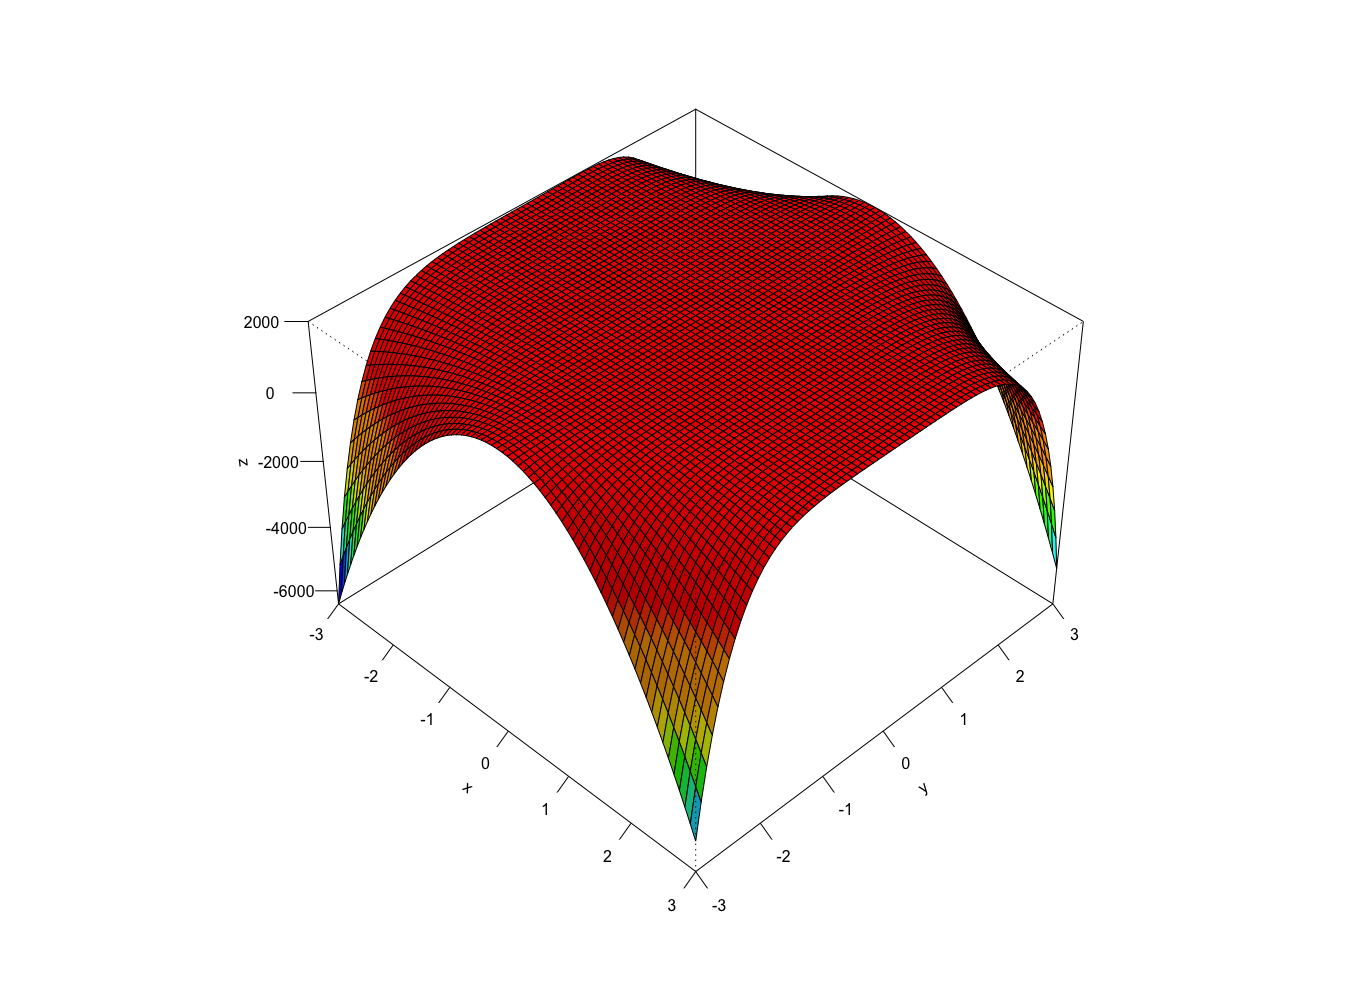
\includegraphics[width= 14cm, height = 14cm]{customizedBeale.png}
	\caption{Customized Beale Function.}
	\label{fig:CustomizedBealeFunction}
\end{figure}

and we picked it up of $2000$ units in order to have as less as possible negative values. So the final adopted function is :

\begin{equation}
f(x, y) = -((1.5 - x + xy)^2 + (2.25 - x + xy^2)^2 + (2.625 - x + xy^3)^2) + 2000
\end{equation}

This customized function has its global maximum in $f(x, y) = 1000$. \\

In order to represent this function using Java Graphical Environment we mapped it in a space of $600 \times 600$ pixels and we properly rotated it. The resulting contour plot is the one represented in figure ~\ref{fig:ContourPlotCustomizedBealeFunction} 

\begin{figure}[h!]
	\centering
	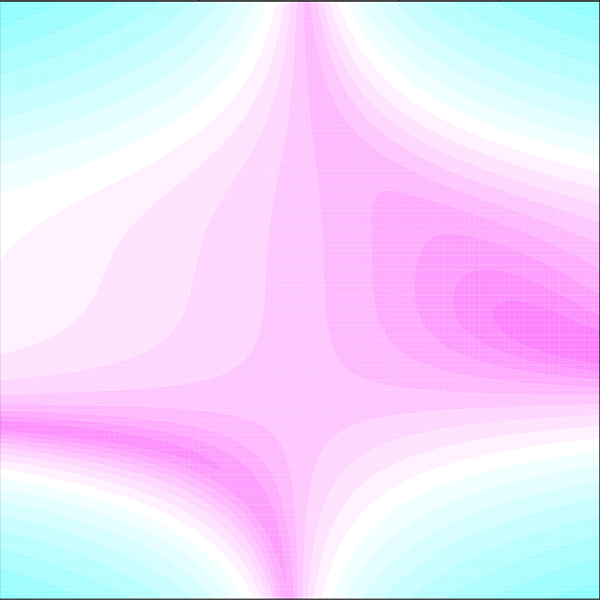
\includegraphics[width= 9cm, height = 9cm]{beale.png}
	\caption{Contour plot of customized Beale Function.}
	\label{fig:ContourPlotCustomizedBealeFunction}
\end{figure}

\subparagraph{Styblinski-Tang Revised Function} In mathematical optimization, Styblinski-Tang Function is a continuous, multi-modal function defined on a multi-dimensional space. The original function is defined by :

\begin{equation}
	f(x) = \dfrac{\sum_{i=1}^{n} x_{i}^4 -16x_{i}^2 +5x_{i}}{2}
\end{equation}

In this thesis we consider the bivariate version of the original function multiplied by two in order to make it less flattened :

\begin{equation}
f(x, y) = (x^4 - 16x^2 + 5x) + (y^4 - 16y^2 + 5y).
\end{equation}

\begin{figure}[h!]
	\centering
	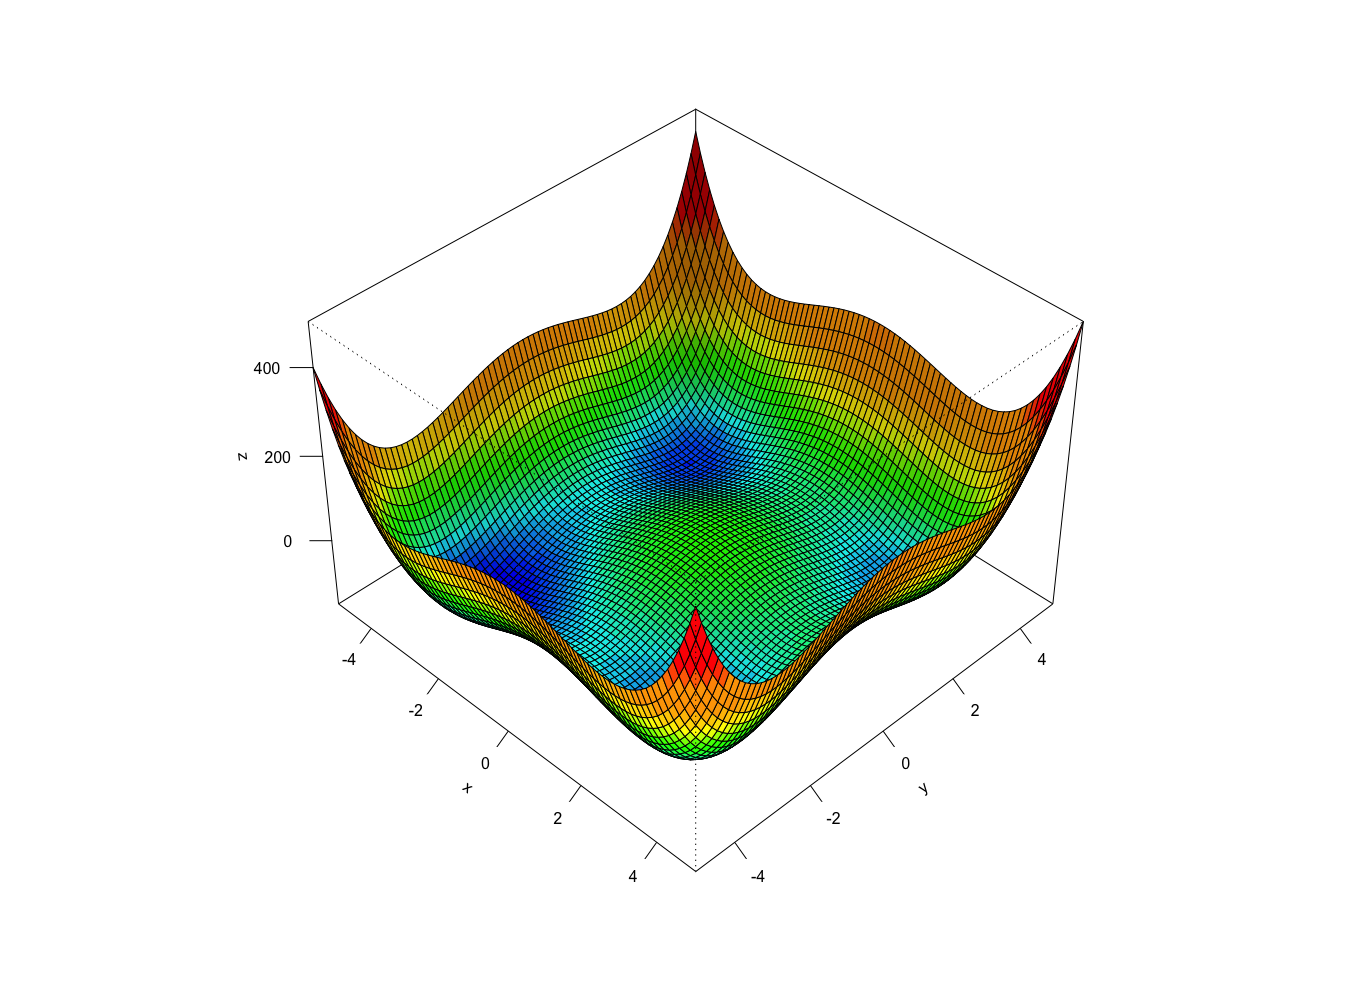
\includegraphics[width= 14cm, height = 14cm]{classicalStyblinski.png}
	\caption{Original Styblinski Function.}
	\label{fig:OriginalStyblinskiFunction}
\end{figure}

The function can be defined on any input domain but it is usually evaluated on $x \in [-5, 5]$ and $y \in [-5, 5]$. \\

In this thesis our aim is to maximize. In order to do this we inverted the function as

\begin{equation}
f(x, y) = -((x^4 - 16 * x^2 + 5 * x) + (y^4 - 16 * y^2 + 5 * y))
\end{equation}

\begin{figure}[h!]
	\centering
	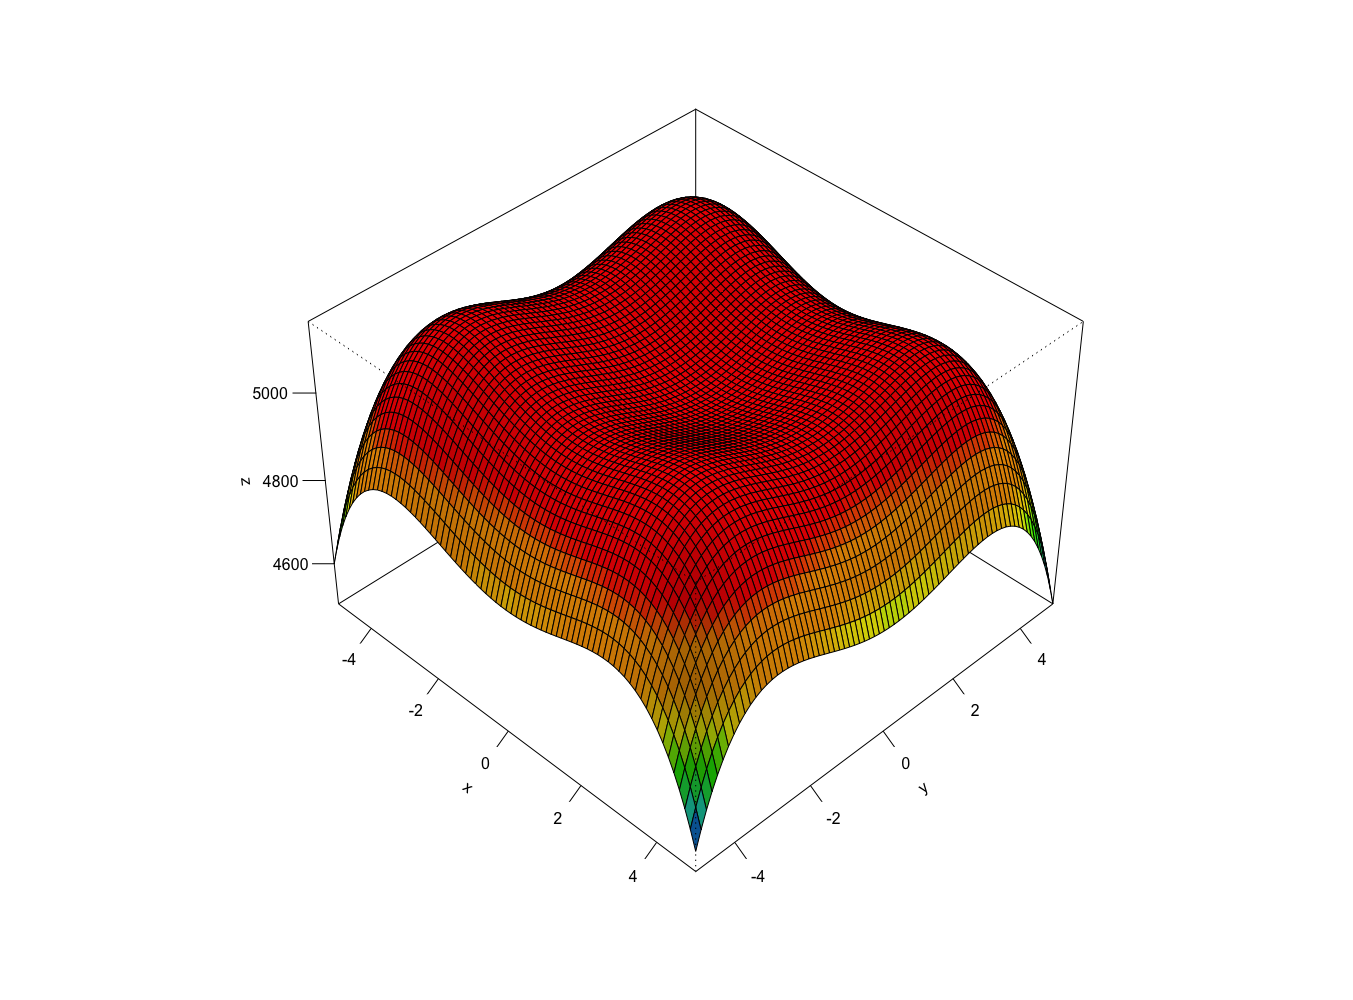
\includegraphics[width= 14cm, height = 14cm]{customizedStyblinski.png}
	\caption{Customized Styblinski Function.}
	\label{fig:CustomizedStyblinskiFunction}
\end{figure}

and we picked it up of $5000$ units in order to has as less as possible negative values. So the final adopted function is: 

\begin{equation}
f(x, y) = -((x^4 - 16 * x^2 + 5 * x) + (y^4 - 16 * y^2 + 5 * y)) + 5000
\end{equation}

This customized function has its global maximum in $f(x, y) = 5156.6638$.

In order to represent this function using Java Graphical Environment we mapped its in a space of $600 \times 600$ pixels and we properly rotated its. The resulting contour plot is the one represented in figure ~\ref{fig:ContourStyblinskiFunction}.

\begin{figure}[h!]
	\centering
	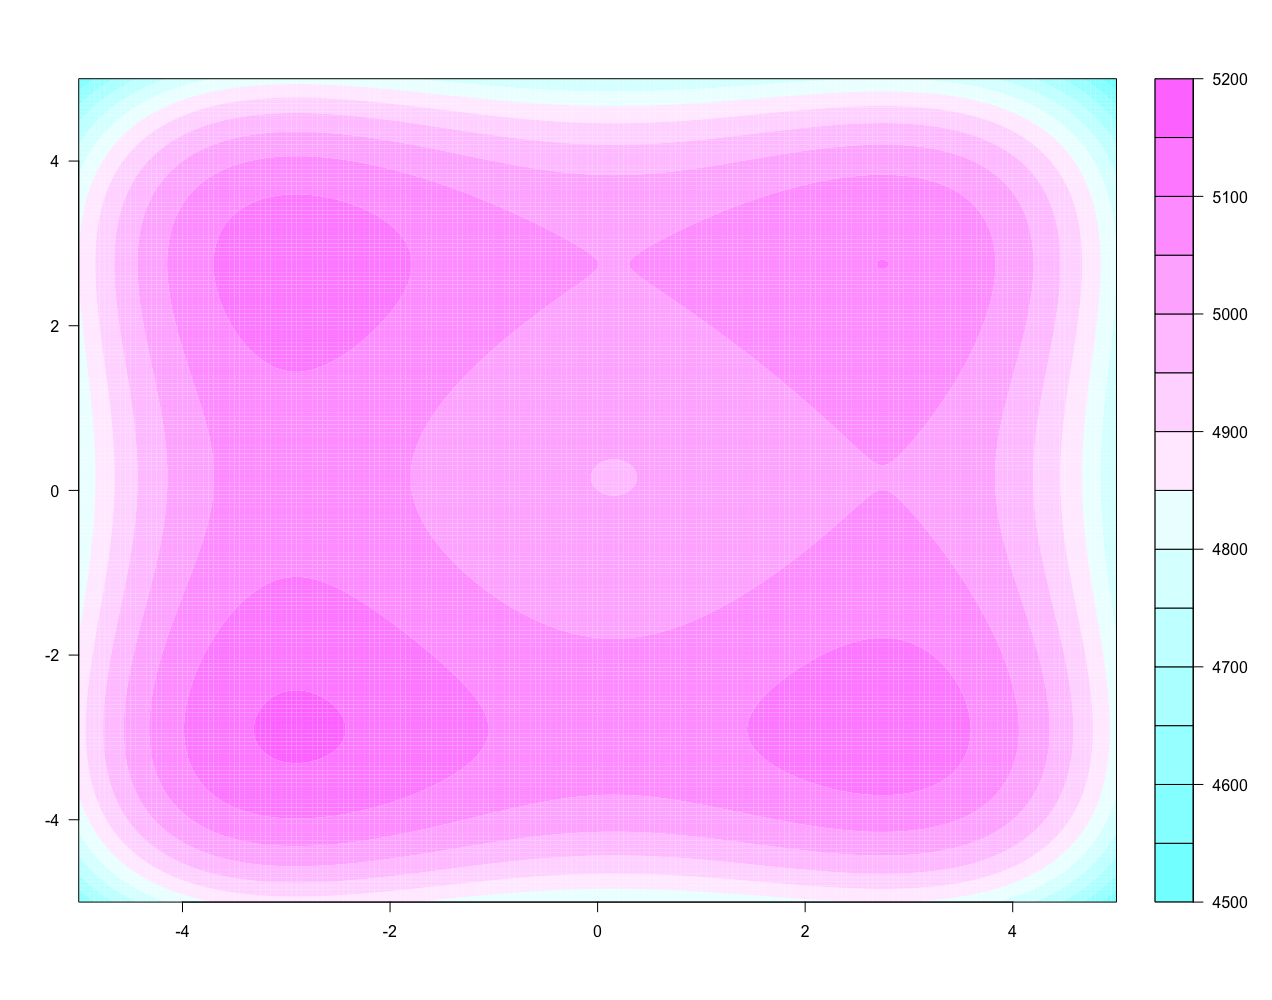
\includegraphics[width= 9cm, height = 9cm]{styblinski.png}
	\caption{Contour plot of customized Styblinski Function.}
	\label{fig:ContourStyblinskiFunction}
\end{figure}






